\documentclass[10pt,a4paper]{report}
\usepackage[utf8]{inputenc}
\usepackage{url}
\usepackage[english]{babel}
\usepackage{amsmath}
\usepackage{amsfonts}
\usepackage{amssymb}
 \usepackage{float}
\usepackage{graphicx}
\usepackage[left=2cm,right=2cm,top=2cm,bottom=2cm]{geometry}
\author{Andres Chaves}
\title{Report 1: Data Analysis}

\begin{document}
 \title{Report 1: Data Description and Analysis}
 \author{Andres Chaves (706801) \\
  \multicolumn{1}{p{.7\textwidth}}{\centering{achaves@student.unimelb.edu.au\\}\centering\emph{Melbourne School of Information\\The University of Melbourne}}}
 \maketitle

\begin{abstract}
    The purpose of this document is to describe and analyse the available data from which the experiments will be executed.
   \\\\
   Throughout this document we will understand what is the data, how much data is available and we will see some examples of relations between the data.
\end{abstract}

 \chapter*{Introduction}
The purpose of my Research Project is to explore how Machine Learning technologies can be used for aiding the Network Management process, specifically the Fault Management process.
\\\\
One of the key Information Technology components in Fault Management is the Fetwork Management System (FMS). A FMS is a system which receives all the alarms from the different Network Elements (NEs), performs several data transformation, and at the end stores an enriched alarm and allows their visualisation:

\begin{figure}[H]
 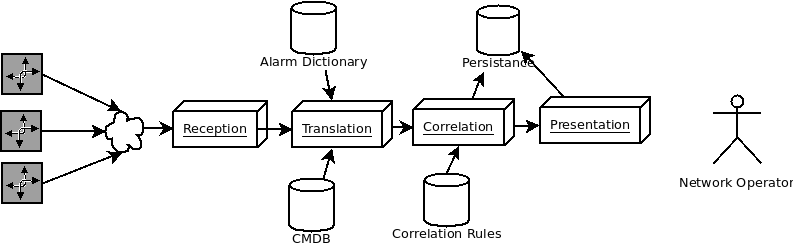
\includegraphics[scale=0.4]{../research_proposal/NMS_GeneralDiagram.png}
  \centering
  \caption{\textit{A schematic of a generic Fault Management System}}
  \label{fig:nms_generaldiagram}
\end{figure}	

The processing stages might include the following:

\begin{itemize}
\item Translation: Consist on receive the alarm in a given standard, de-codify it, translate it and enrich it into useful data. This is a required step.

\item Correlation: Consist on establish rules for alarm suppression and correlation to present only key information to the network operator.
\end{itemize}

In order to conduct the experiment and analysis the candidate data will be the one stored by the NMS and for the experiments I will use the data of a specific  NMS built in one of the  companies I formerly worked on.

\chapter{Simple Network Management Protocol SNMP}
- Protocol RFC, year
- MIB, Trap, information, bindings, oid

\chapter{Fault Management System}

Based on the overall components of a generic FMS in Figure \ref{fig:nms_generaldiagram}, in the former company I worked for, we built a specific FMS using several Open Source software. 

\begin{figure}[H]
 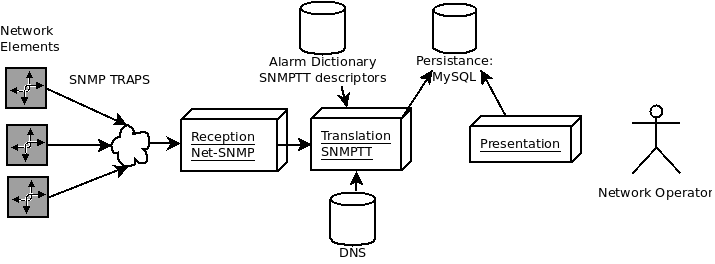
\includegraphics[scale=0.4]{ACC_FMS.png}
  \centering
  \caption{\textit{Our built Fault Network Management System}}
  \label{fig:acc_fms}
\end{figure}	


The FMS receives alarms using the SNMP protocol\cite{snmp}. The Open Source components used are described as follows:

\begin{itemize}
  \item Net-SNMP: Net-SNMP is an open source Linux and Unix package that implements the SNMP protocol. The role of this component will be the reception of alarms by using the snmptrapd daemon\cite{netsnmp}.
  \item SNMPTT: SNMPTT or SNMP-Trap Translator is an open source component that takes the SNMP trap (alarm) received by Net-SNMP and by using an alarm dictionary (to interpret the alarm name and its attributes) and a DNS (to gather the NE name) translates it into a more useful event. SNMPTT can also enrich the alarm from a database by executing a shell script.\cite{snmptt}
  \item MYSQL: MySQL is an open source relational database. For this project, it will be used as storage of the Alarms and Configuration Management Database\cite{mysql}.
\end{itemize}

\chapter{Network Description}
 layers (AC, AG, CN), elements in a Node, Suppliers
\subsection{Host Naming Convention}
It is important to describe the host naming convention used for the network elements because it provides useful information. A host name is a 19 character string which follows the convention NEROLE\_BRAND\_MODEL\_STATE\_TOWN\_CONSECUTIVE (i.e: AC\_ER\_SP10\_ST\_VCH\_1):

\begin{itemize}
   \item Network Element Role: Two letters that correspond to the type of node where the network element is located. The type of node can be AC (Access), AG (Agregator), CN (Concentrator), CR (CORE), IG (Internet Gateway) and RC (Rectifier).
   \item Brand: Two letters that correspond to the fabricator name of the equipment. Somes examples are: ER, AL, DT.
   \item Model: Four letters that codifies to the NE's model. Some examples are: SP10, SA30, DP29.
   \item State: Two letters that represents the state where the network element is physically located.
   \item Town: Three letters encoding the town where the network element is physically located.
\end{itemize}

 
\chapter{Data Specification}

The FMS specified in the last section stores the alarms in a table on a Relational Database System. Each month of alarms is stored in a separated table. For the purpose of this analysis we used the table for the month of October, 2014.

\section{Data Attributes}

The relevant attributes of the alarms stored are:

\begin{itemize}
  \item Id: Unique numeric identifier of each alarm.
  \item Eventname: Correspond to the translated name of the alarm's OID as informed by the SNMPTT dictionary.
  \item Traptime: Timestamp of arrival of the trap.
  \item Hostname: Ip or host name of the entity that sends the alarm. A DNS is queried in order to translate the IP Address, if the translation is successful the name is stored otherwise the ip is inserted. Most of the host names follow a naming convention.
  \item Formatline: Semi-structured formatted line of the alarm. Normally it includes all the alarm's trap bindings.
\end{itemize}

\begin{figure}[H]
 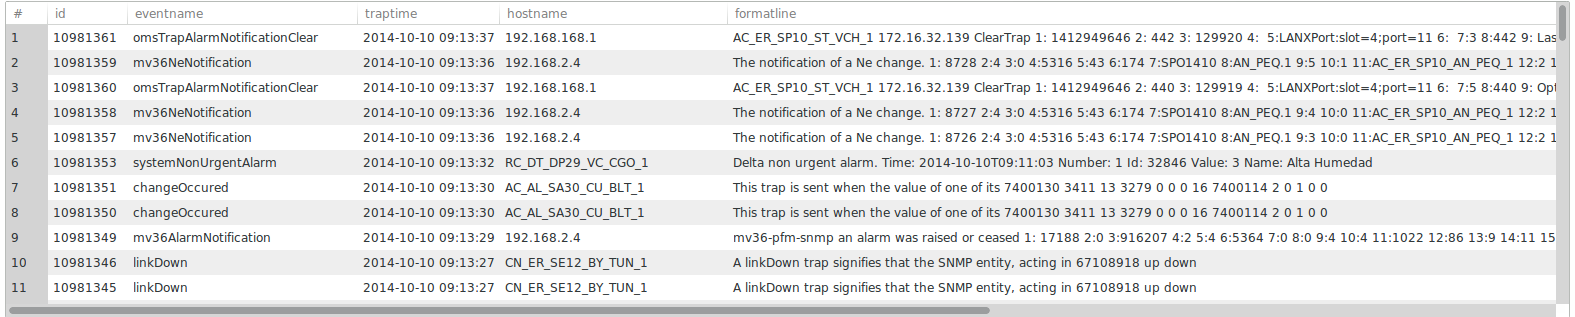
\includegraphics[scale=0.4]{alarms_db_sample.png}
  \centering
  \caption{\textit{An example of the stored data}}
  \label{fig:acc_dataexample}
\end{figure}	

\section{Data Overview} 
For this particular month of October 2014 we have the following overall information:

\begin{center}
 \begin{tabular}{||c | c ||} 
 \hline\hline
 Total Alarms  & 2350714 \\ 
 \hline
 Different Alarm Types & 351 \\ 
 \hline
 Different Host Names & 3272 \\
  \hline
 Average of Alarms Received per Minute & 53 \\
 \hline
 Peak of Alarms Received in a Minute & 714 \\
 \hline\hline
\end{tabular}
\end{center}

\section{Data Analysis} 
In order to have a better insight of the data and to understand better what should be the work required by the learning algorithm, we described 5 different examples of correlation between two alarms.
\\\\
For each correlation example we established the statistical frequency of, in a time window of 1 minute, what is the occurrence of alarm T1, the occurrence of the alarm T2, the occurrence of the alarm T1 given the occurrence of the alarm T1.
\\\\\
\(\forall x \in X, \quad \exists y \leq \epsilon\)
The following table summarises the frequencies:

\begin{center}
 \begin{tabular}{||c | c | c | c ||} 
 \hline\hline
 Scenario  & P(at) & P(a2) & P(a2|at) \\ 
 \hline
 AC Outage + Link Down & 0.2214 & 0.3886 & 0.11 \\ 
 \hline\hline
\end{tabular}
\end{center}

\subsection{Scenario 1: AC Outage + Link Down, Fabricator 1} 
\subsection{Scenario 2: AC Recovery + Link Up, Fabricator 1} 
\subsection{Scenario 3: AC Outage + Link Down, Fabricator 2} 
\subsection{Scenario 4: AC Recovery + Link Up, Fabricator 2} 
\subsection{Scenario 5: Fuse Breaker Alarm + Link Down, Fabricator 1} 

 \begin{thebibliography}{9}
\bibitem{snmp}IETF RFC 1157, \url{http://www.ietf.org/rfc/rfc1157.txt?number=1157}.
\bibitem{netsnmp}Net-SNMP website, \url{http://www.net-snmp.org/}.
\bibitem{snmptt}SNMPTT website, \url{http://snmptt.sourceforge.net/docs/snmptt.shtml}.
\bibitem{mysql}MySQL website, \url{http://dev.mysql.com/doc/refman/4.1/en/what-is-mysql.html}.

 
\end{thebibliography}
    
\end{document}
